\section{Muon System}

Muon detection is an important requirement for the LHCb detector. Muons are present in the final state of many of the key decays that are sensitive to new physics and the rare decays shown in table \ref{table: Muon decays}, They are also used to determine the flavour of neutral B mesons in electroweak and strong processes.% in in $B_{d,s}^0 \rightarrow \mu X$ decays.


%\begin{itemize}
%	\item $B_s^0 \rightarrow \mu^+ \mu^-$ %[First evidence for the decay Bs -> mu+ mu-]}
%	 \item $B \rightarrow J/\psi(\mu^+\mu^-)K_s$ %[Measurement of the isospin asymmetry in $B \to K^{(*)}?^+?^-$ decays]
%	 \item $B_s^0 \rightarrow J/\psi(\mu^+\mu^-)\Phi$ %[Measurement of the CP-violating phase phi_s in the decay Bs->J/psi phi]
% \end{itemize}
% 
% \begin{equation*}
%	B_s^0 \rightarrow \mu^+ \mu^-
%\end{equation*}
% 
% \begin{equation*}
%	B_s^0 \rightarrow \mu^+ \mu^-
%\end{equation*}
% 
% \begin{equation*}
%	B_s^0 \rightarrow \mu^+ \mu^-
%\end{equation*}

\begin{table*}[htdp]
	\caption{}
	\begin{center}
		\begin{tabular}{|c|}
			\hline
			Process \\ 
			\hline
			$B_s^0 \rightarrow \mu^+ \mu^-$ \\
			$B \rightarrow J/\psi(\mu^+\mu^-)K_s$ \\ 
			$B_s^0 \rightarrow J/\psi(\mu^+\mu^-)\Phi$ \\
			\hline
		\end{tabular}
	\end{center}
	\label{table: Muon decays}
\end{table*}%

To reconstruct these types of events at the LHCb bunch crossing rate (which peaks at 40MHz corresponding to a bunch crossing every 25 ns) the muon system employs a fast stand alone muon reconstruction and passes the information to the hardware trigger (see section \ref{section: trigger}) of the LHCb which applies a minimum $p_T$ requirement (1.5 GeV/c for events with a single muon or a geometrical mean of 1.3 GeV/c for the two muons with the highest $p_T$ in the event). Events triggered on this muon requirement make up $\sim40\%$ of the hardware level trigger output; together with data from the calorimeter system this makes up the bulk.

For the LHCb detector to be competitive in the physics analysis of decays such as shown in table \ref{table: Muon decays} a trigger efficiency of $\sim95\%$, muon identification of $\sim90\%$, muon misidentification of $\sim1.5\%$ and muon $p_T$ resolution of $\sim20\%$ is required 
%[Muon TDR 2001]
together with a timing resolution of $\sim25$ ns to match the nominal bunch crossing rate. In addition to this the hardware must be capable of handling the high rates of particles passing through the detector as well as the associated radiation damage.

%\begin{table*}[htdp]
%	\begin{center}
%		\caption{$B\rightarrow \mu X$ background processes at LHCb}
%		\begin{tabular}{|c|}
%			\hline
%			Example Background Processes \\
%			\hline
%			$\pi, K \rightarrow \mu X$ \\
%			Shower particles from the calorimeter system \\
%			Machine background, in particular high energy beam halo muons \\
%			\hline
%		\end{tabular}
%	\end{center}
%	\label{table: muon background}
%\end{table*}%

The Muon System is made up of five stations orientated perpendicularly to the beam axis; these are named M1 through to M5, each consisting of two mechanically independent halves called the A and C side. M1 is positioned before the Pre Shower of the calorimeter system 12.1 m from the nominal interaction point and stations M2-M5 are positioned downstream of the calorimeter system 15.2 m, 16.4 m, 17.6 m and 18.8 m from the interaction point (figure \ref{fig: muon system layout}). Stations M2-M5 are interleaved with 80 cm thick iron absorbers designed to remove hadronic backgrounds giving a longitudinal size of 20 hadron interaction lengths for stations M2-M5 ~\cite{1748-0221-8-02-P02022}. The geometry of the muon stations is projective to the nominal interaction point; the transverse dimensions scale with distance from the nominal interaction point such that the angular acceptance is the same for all muon stations; $\pm 306$mrad in the horizontal plane and $\pm 258$mrad in the vertical plane. 

Each of the muon stations is divided into four rectangular regions, labeled R1-R4 in order of radial distance from the beam axis (Since the geometry of the muon stations is projective to the nominal interaction point the relative sizes of the regions between each station are the same). These are further subdivided into 276 rectangular chambers of varying size depending on in which region the chamber is located (figure \ref{fig: muon region granularity}). The chambers are made up of Multi-Wire Proportional Chambers (MWPC) with the exception of R1 in station M1 which uses triple-GEM detectors(Gas Electron Multiplier) due to higher expected particle rates in this region and the higher levels of radiation tolerance for triple-GEM detectors \cite{muon-second-addemdum}. This gives a total of 1380 chambers providing a detection area of 435 m$^2$.

\begin{figure}[htbp]
	\begin{center}
		\begin{subfigure}[b]{0.45\textwidth}
			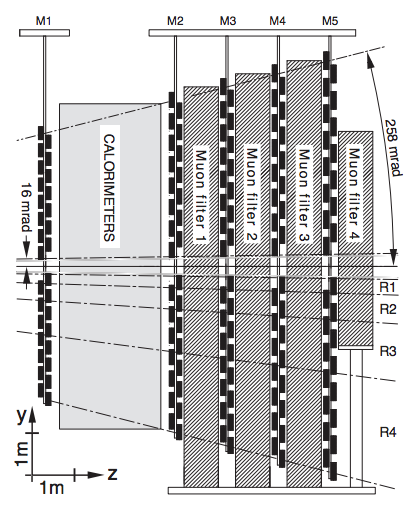
\includegraphics[width=\textwidth]{./Chapters/detector/muon_system/muon_system_side_view.png}
			\caption{Side view of the muon system}
			\label{default}
		\end{subfigure}
		\begin{subfigure}[b]{0.45\textwidth}
			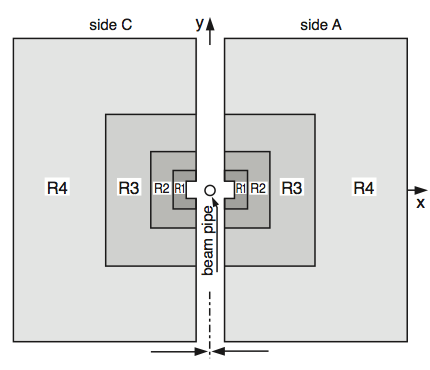
\includegraphics[width=\textwidth]{./Chapters/detector/muon_system/muon_regions.png}
			\caption{Front view of the muon station regions}
			\label{default}
		\end{subfigure}
	\end{center}
	\caption{Muon system layout}
	\label{fig: muon system layout}
\end{figure}

%\begin{table}[htdp]
%	\caption{Particles rates in the muon system, estimated in the Technical Design Report ~\cite{muon-tdr}}
%	\begin{center}
%		\begin{tabular}{|c|c|c|c|c|c|}
%			\hline
%			& M1 & M2 & M3 & M4 & M5 \\
%			\hline
%			R1 & 460 kHz & 37.5 kHz & 10 kHz & 6.5 kHz & 4.4 kHz \\
%			\hline
%			R2 & 186 kHz & 26.5 kHz & 3.3 kHz & 2.2 kHz & 1.8 kHz \\
%			\hline
%			R3 & 80 kHz & 6.5 kHz & 1 kHz & 0.75 kHz & 0.65 kHz \\
%			\hline
%			R4 & 25 kHz & 1.2 kHz & 0.42 kHz & 0.25 kHz & 0.23 kHz \\
%			\hline
%		\end{tabular}
%	\end{center}
%	\label{default}
%\end{table}%

The chambers are further subdivided into logical pads; the dimensions of which vary between muon stations. Stations M1-M3 are used in the muon trigger to calculate the $p_t$ of muon candidates (since muons are more attenuated at the further downstream muon stations) and so the granularity in the bending plane (horizontal) is finer than that of stations M4 and M5 (which are used to identify penetrating muons).

\begin{figure}[htbp]
	\begin{center}
			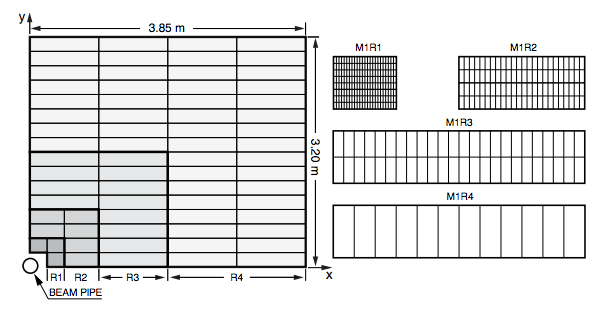
\includegraphics[width=\textwidth]{./Chapters/detector/muon_system/logical_pad_layout.png}
		\caption{On the left is a quadrant of the M1 station with the regions R1-R4 shown. Each rectangle represents a chamber. On the right are the chambers for regions, R1-R4 with the logical pad sub-structure shown}
		\label{fig: muon region granularity}
	\end{center}
\end{figure}

Overall the muon system has performed very well during the operation of LHCb achieving if not exceeding the requirements set by the Technical Design Report \cite{muon-tdr}. In particular efficiencies are well above the design requirements previously described \cite{Alves:2012ey}, see figure; efficiencies and mis Id rates together with the PID information from the RICH detector can be seen in figure \cite{Archilli:2013npa}. The momentum resolution achieved from the stand alone muon system reconstruction is ~25\% and ~0.4\% with the offline reconstruction using the tracking information \cite{Alves:2012ey}.






















